\documentclass{standalone}
\usepackage{tikz}
\usepackage{ctex,siunitx}
\setCJKmainfont{Noto Serif CJK SC}
\usepackage{tkz-euclide}
\usepackage{amsmath}
\usetikzlibrary{patterns, calc,3d}
\usetikzlibrary {decorations.pathmorphing,decorations.pathreplacing,decorations.shapes,}
\tikzset{label style/.append style={font=\small}}
\begin{document}
\small
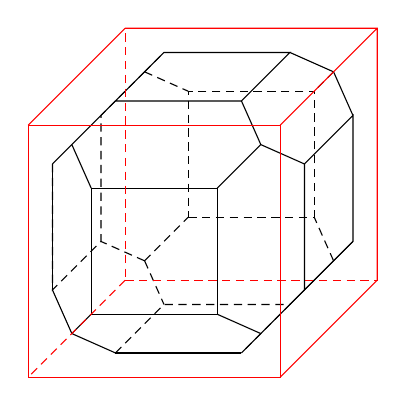
\begin{tikzpicture}[>=latex,scale=0.8]
  \draw[densely dashed](1,1,0)--(3,1,0)--(3,3,0)--(1,3,0)--cycle;
  \draw(1,1,4)--(3,1,4)--(3,3,4)--(1,3,4)--cycle;
  \draw[densely dashed](1,0,3)--(1,0,1)--(3,0,1)--(3,0,3);
  \draw(1,0,3)--(3,0,3);
  \draw(1,4,1)--(3,4,1)--(3,4,3)--(1,4,3)--cycle;
  \draw(0,3,3)--(0,1,3);
  \draw[densely dashed](0,3,3)--(0,1,3)--(0,1,1)--(0,3,1);
  \draw(4,1,1)--(4,3,1)--(4,3,3)--(4,1,3)--cycle;
  \draw(3.5,3.5,3.5)--(3,3,4)(3.5,3.5,3.5)--(3,4,3)(3.5,3.5,3.5)--(4,3,3);
  \draw(3.5,3.5,0.5)--(3,4,1)(3.5,3.5,0.5)--(4,3,1);
  \draw[densely dashed](3.5,3.5,0.5)--(3,3,0);
  \draw(0.5,3.5,3.5)--(1,3,4)(0.5,3.5,3.5)--(1,4,3)(0.5,3.5,3.5)--(0,3,3);
  \draw(0.5,0.5,3.5)--(1,1,4)(0.5,0.5,3.5)--(1,0,3)(0.5,0.5,3.5)--(0,1,3);
  \draw(3.5,0.5,0.5)--(3,0,1)(3.5,0.5,0.5)--(4,1,1);
  \draw[densely dashed](3.5,0.5,0.5)--(3,1,0);
  \draw(3.5,0.5,3.5)--(3,1,4)(3.5,0.5,3.5)--(3,0,3)(3.5,0.5,3.5)--(4,1,3);
  \draw[densely dashed](0.5,0.5,0.5)--(1,1,0)(0.5,0.5,0.5)--(1,0,1)(0.5,0.5,0.5)--(0,1,1);
  \draw[densely dashed](0.5,3.5,0.5)--(1,4,1)(0.5,3.5,0.5)--(1,3,0)(0.5,3.5,0.5)--(0,3,1);
  \draw[densely dashed,red](0,0,0)--(4,0,0)--(4,4,0)--(0,4,0)--cycle;
  \draw[red](0,0,4)--(4,0,4)--(4,4,4)--(0,4,4)--cycle;
  \draw[densely dashed,red](0,0,0)--(0,0,4);
  \draw[red](0,4,0)--(0,4,4)(4,4,0)--(4,4,4)(4,0,0)--(4,0,4)(0,4,0)--(4,4,0)--(4,0,0);
\end{tikzpicture}
\end{document}